\documentclass[t]{beamer}
% Source: https://www.overleaf.com/latex/templates/vse-fmv-presentation-template/bnwxsdjhjkvv

\usetheme{Madrid}

% Custom green
\definecolor{MyGreen}{RGB}{0,120,80}  % dark professional green

\usecolortheme[named=MyGreen]{structure}

\setbeamercolor{palette primary}{bg=MyGreen,fg=white}
\setbeamercolor{palette secondary}{bg=MyGreen!80!black,fg=white}
\setbeamercolor{palette tertiary}{bg=MyGreen!60!black,fg=white}

\setbeamerfont{caption}{size=\footnotesize}


% Packages
\usepackage[utf8]{inputenc}
\usepackage{hyperref}
\usepackage{tikz} 
\usepackage{booktabs}
\usepackage{natbib}

% --- 1. CONFIGURATION FOR CONTENT SLIDES (Middle Pages) ---
\addtobeamertemplate{frametitle}{}{%
    \begin{tikzpicture}[remember picture,overlay]
        \node[anchor=north east, xshift=-0.3cm, yshift=0cm, inner sep=0pt] at (current page.north east) {
            
\includegraphics[height=0.8cm, keepaspectratio]{logo_1}
        };
    \end{tikzpicture}%
}

% --- 2. CONFIGURATION FOR FIRST & LAST PAGE ---
\newcommand{\FirstLastPageLayout}{
    \begin{tikzpicture}[remember picture,overlay]
        \node[anchor=north east, xshift=-0.3cm, yshift=0cm, inner sep=0pt] at (current page.north east) {
            
\includegraphics[height=1cm, keepaspectratio]{logo_2}
        };
%        \node[anchor=south west, xshift=0.5cm, yshift=0.5cm] at (current page.south west) {
%            \textcolor{MyGreen}{\footnotesize Prague University of Economics and Business}
%        };
    \end{tikzpicture}
}

% --- Info ---
\title[Title]{QPM Technical Training} % 
%\subtitle{Subtitle of your presentation} % 
\author{name} % 
\institute[]{Institution} % 
\date{\today}

\begin{document}

% --- Slide 1: Title Page ---
\begin{frame}
    \FirstLastPageLayout % 
    \titlepage
\end{frame}

% --- Slide 2: Contents ---
\begin{frame}{Contents} % 
    \begin{itemize}
        \item Motivation % 
        \item Research gap \& Aim of the paper % 
        \item Theoretical background
        \item Methodology
        \item Results \& Discussion
        \item Further research \& Limitations  
    \end{itemize}
\end{frame}

% --- Motivation ---
\begin{frame}{Motivation} % 
    \begin{itemize}
        \item \textbf{XYZ} – your text % 
        
        \vspace{0.2cm}
        \footnotesize{\textit{(...your text)}} % 
        \vspace{0.2cm}
        \normalsize
        
        \item \textbf{XYZ} - your text % 
        \begin{itemize}
            \item tbc % 
        \end{itemize}
        
        \item ... % 
      

    \end{itemize}
\end{frame}

% --- Research gap \& Aim of the paper ---
\begin{frame}{Research gap \& Aim of the paper} % 
    \begin{itemize}
        \item To insert a table...
    \end{itemize}
    \begin{table}[h!]
\centering
\caption{Summary statistics of XX} \label{HHI_table}
\begin{tabular}{lrrr}
\hline
Country & Mean X & Min X & Max X \\
\hline
AT & 0.29 & 0.28 & 0.30  \\
BE & 0.27 & 0.25 & 0.29 \\
BG & 0.23 & 0.20 & 0.28 \\
\hline
\multicolumn{4}{@{}l} {\tiny Source: own elaboration based on }
\end{tabular}
\end{table}
\end{frame}

% --- Theoretical background ---
\begin{frame}{Theoretical background} % 
    \begin{itemize}
        \item To insert an equation...
    \end{itemize}
    \begin{equation}
        Y = \beta_0 + \beta_1 X + \epsilon
    \end{equation}
\end{frame}

% --- Methodology ---
\begin{frame}{Methodology} % 
    \begin{itemize}
        \item Your text
    \end{itemize}
\end{frame}

% --- Data ---
\begin{frame}{Data} % 
    \begin{itemize}
        \item Your text
    \end{itemize}
\end{frame}

% --- Results \& Discussion ---
\begin{frame}{Results \& Discussion} % 
    \begin{itemize}
        \item To include a figure...
    \end{itemize}

    \begin{figure}
                \caption{XYZ}
             
                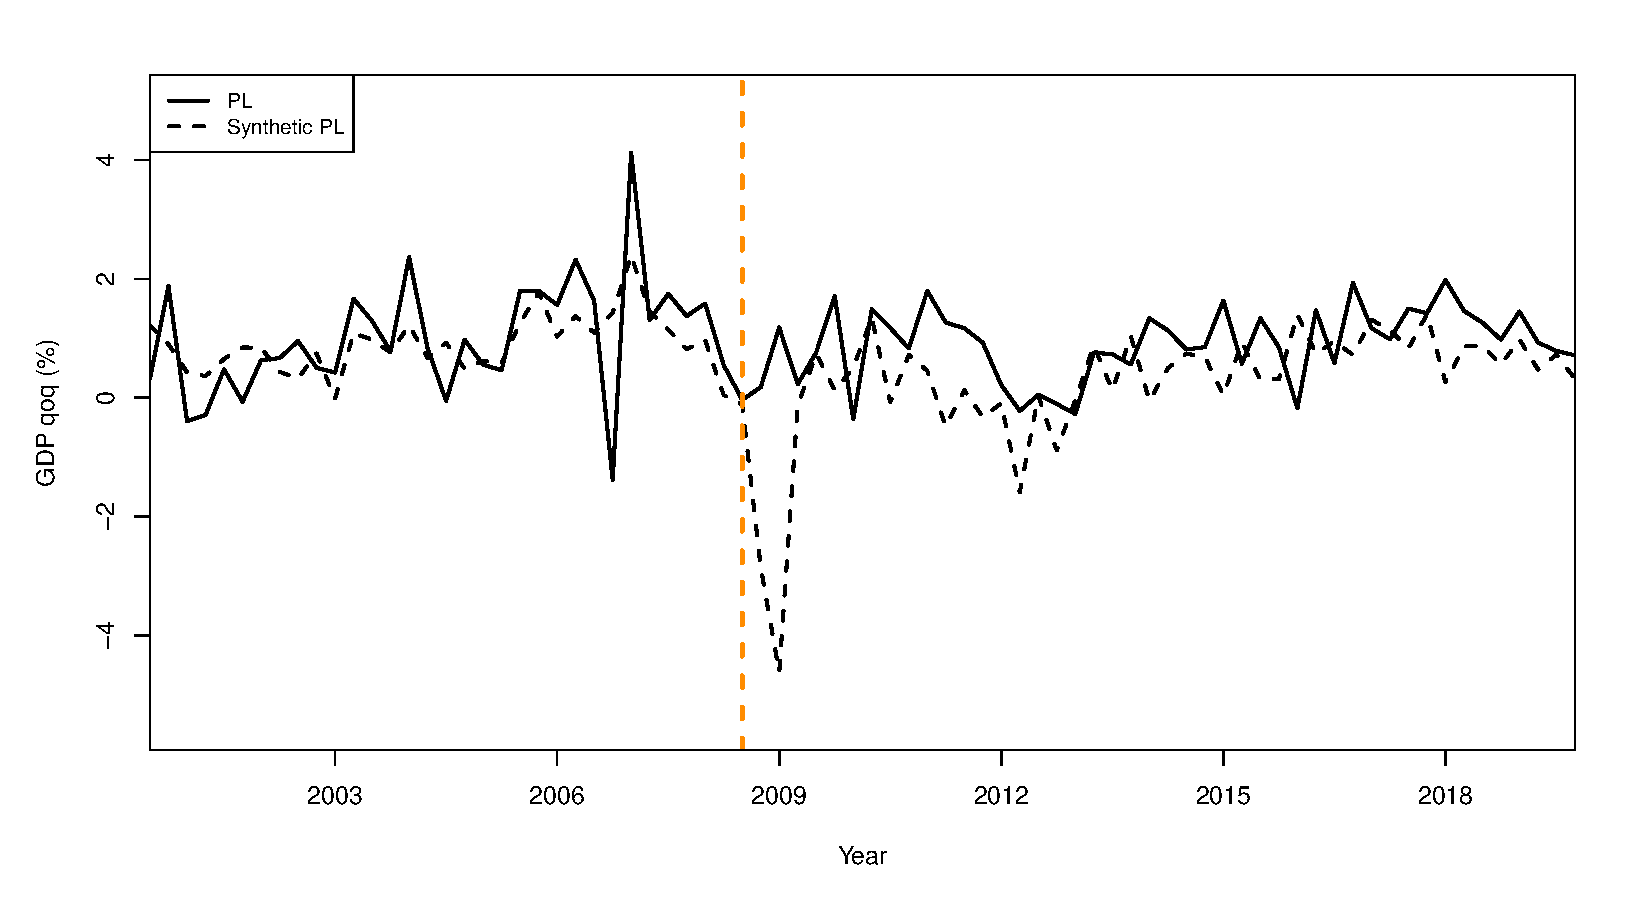
\includegraphics[width=7cm]{PL_GDP.pdf}
                
                {\tiny Source: Authors' calculations}
            \end{figure}

\end{frame}

% --- Further research \& Limitations ---
\begin{frame}{Further research \& Limitations} % 
    \begin{itemize}
        \item Your text
    \end{itemize}
\end{frame}

% --- References ---

\begin{frame}[allowframebreaks]{References}

\tiny
\bibliography{references}
\bibliographystyle{apalike}

\end{frame}

% --- Final page ---
\begin{frame}[c]
    \FirstLastPageLayout % 
    \centering
    \Huge \textcolor{MyGreen}{Thank you for your attention} % 
    
    \vspace{1.5cm}
    \normalsize
    \textbf{Your Name} \\ % 
    \href{mailto:your.email@vse.cz}{your.email@vse.cz} % 
\end{frame}


\end{document}